\subsection{(W) Avoidance grid run}\label{s:aviudabceGridRun}
    \begin{itemize}
        \item Avoidance grid and data fusion procedure (sensor/information source)
        \item Obstacle rating calculation - visibility, map, constraints, detected obstacles, long term weather
        \item Intruder rating calculation - intruder intersection models, dynamic constraints, short term weather
        \item Reachibility rating calculation for trajectory
        \item Reachibility rating for cell calculation
        \item Feasible avoidance cells selection process
        \item Waver procedure - when something goes wrong
		\item Low cost sensor fusion \cite{sabatini2013low}.
		\item Concat trajectory search semioptimal like ours \cite{shaw1998using}.
    \end{itemize}
    \begin{figure}[H]
    \centering
        \begin{subfigure}{0.48\textwidth}
            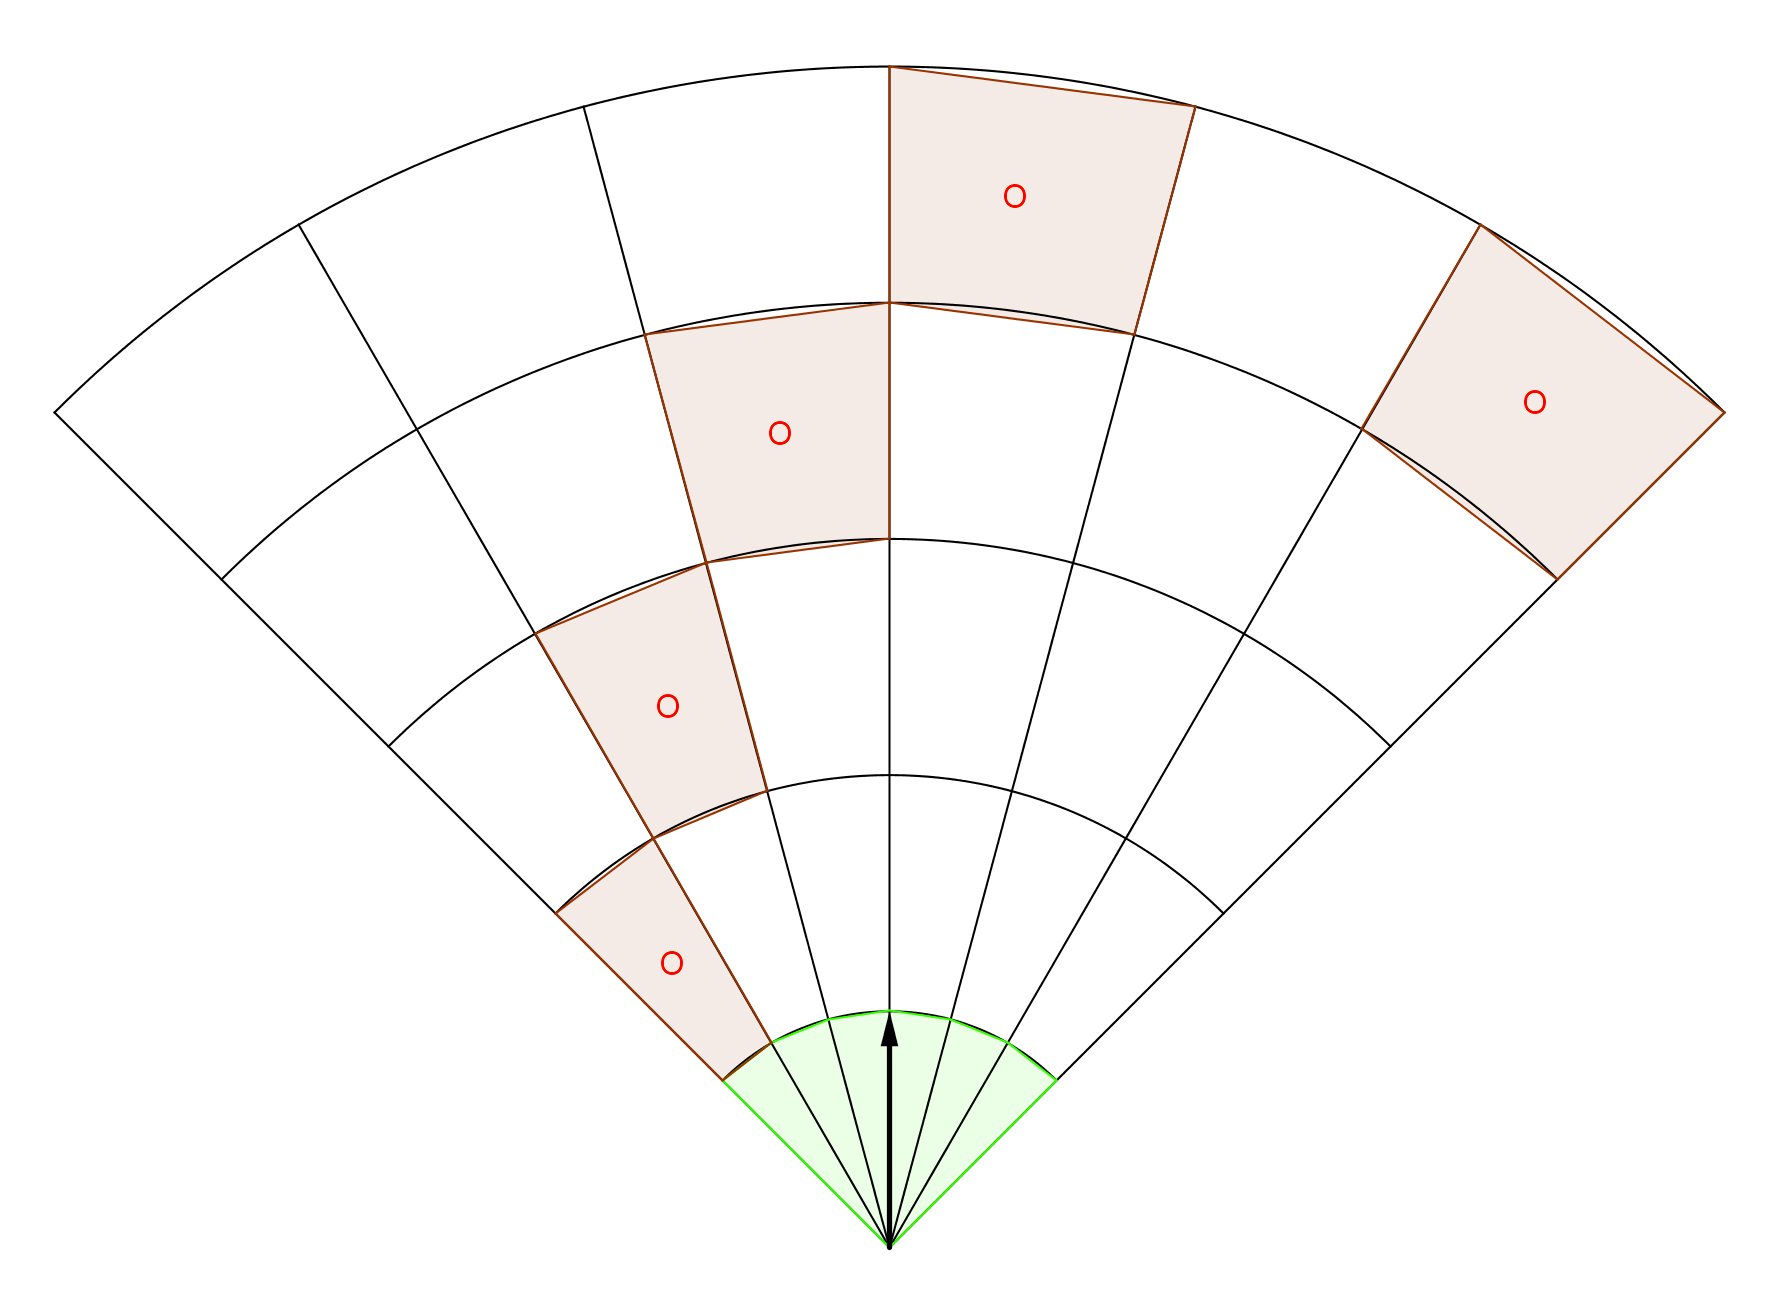
\includegraphics[width=0.9\linewidth]{\FIGDIR/CA001ObstacleDetection}
            \caption{Obstacle detection.}
            \label{fig:obstacleDetectionAvoidanceGrid}
        \end{subfigure}
        \begin{subfigure}{0.48\textwidth}
            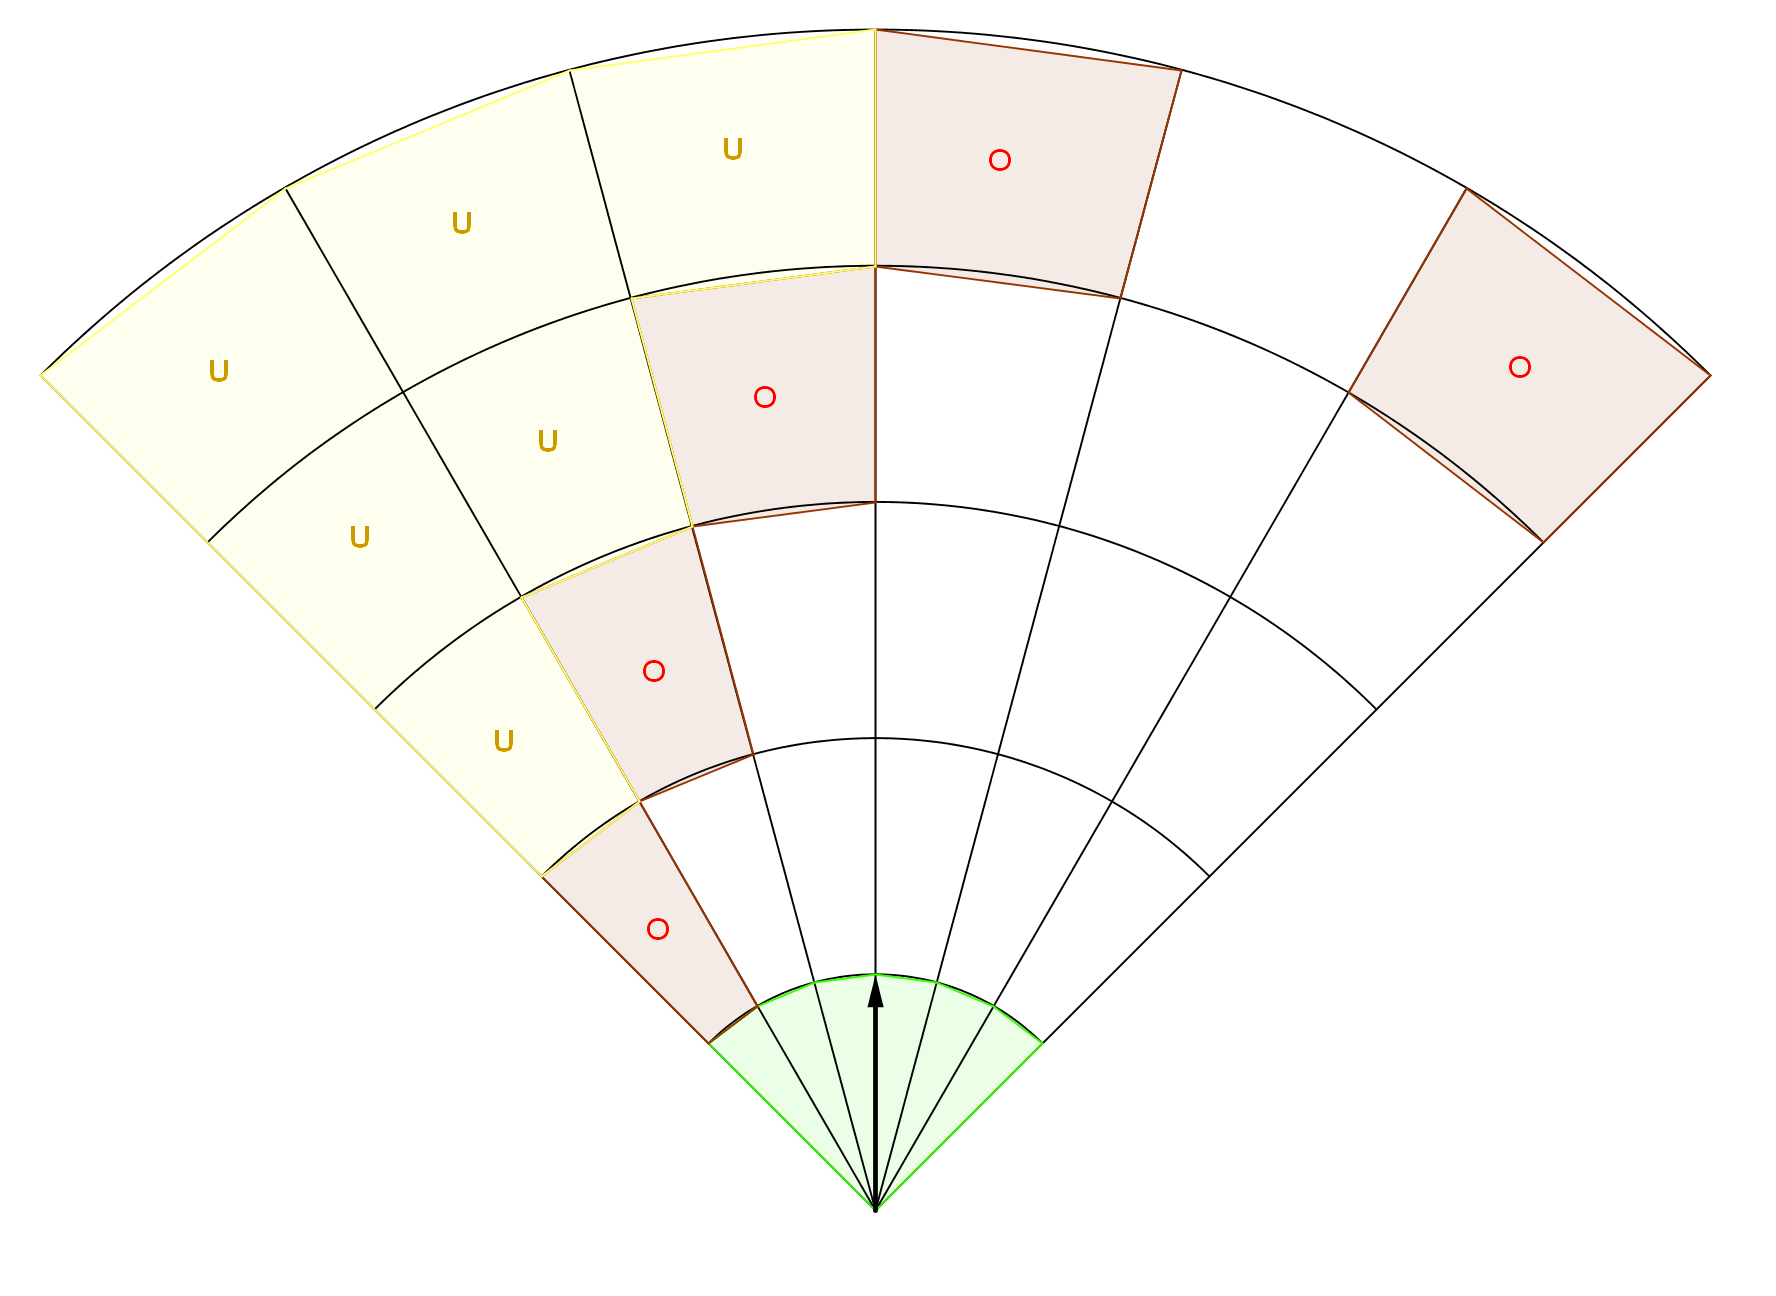
\includegraphics[width=0.9\linewidth]{\FIGDIR/CA002UncertainityAssesment} 
            \caption{Uncertainty assessment.}
            \label{fig:uncertainityAssesmentAvoidanceGrid}
        \end{subfigure}
        \\
        \begin{subfigure}{0.48\textwidth}
            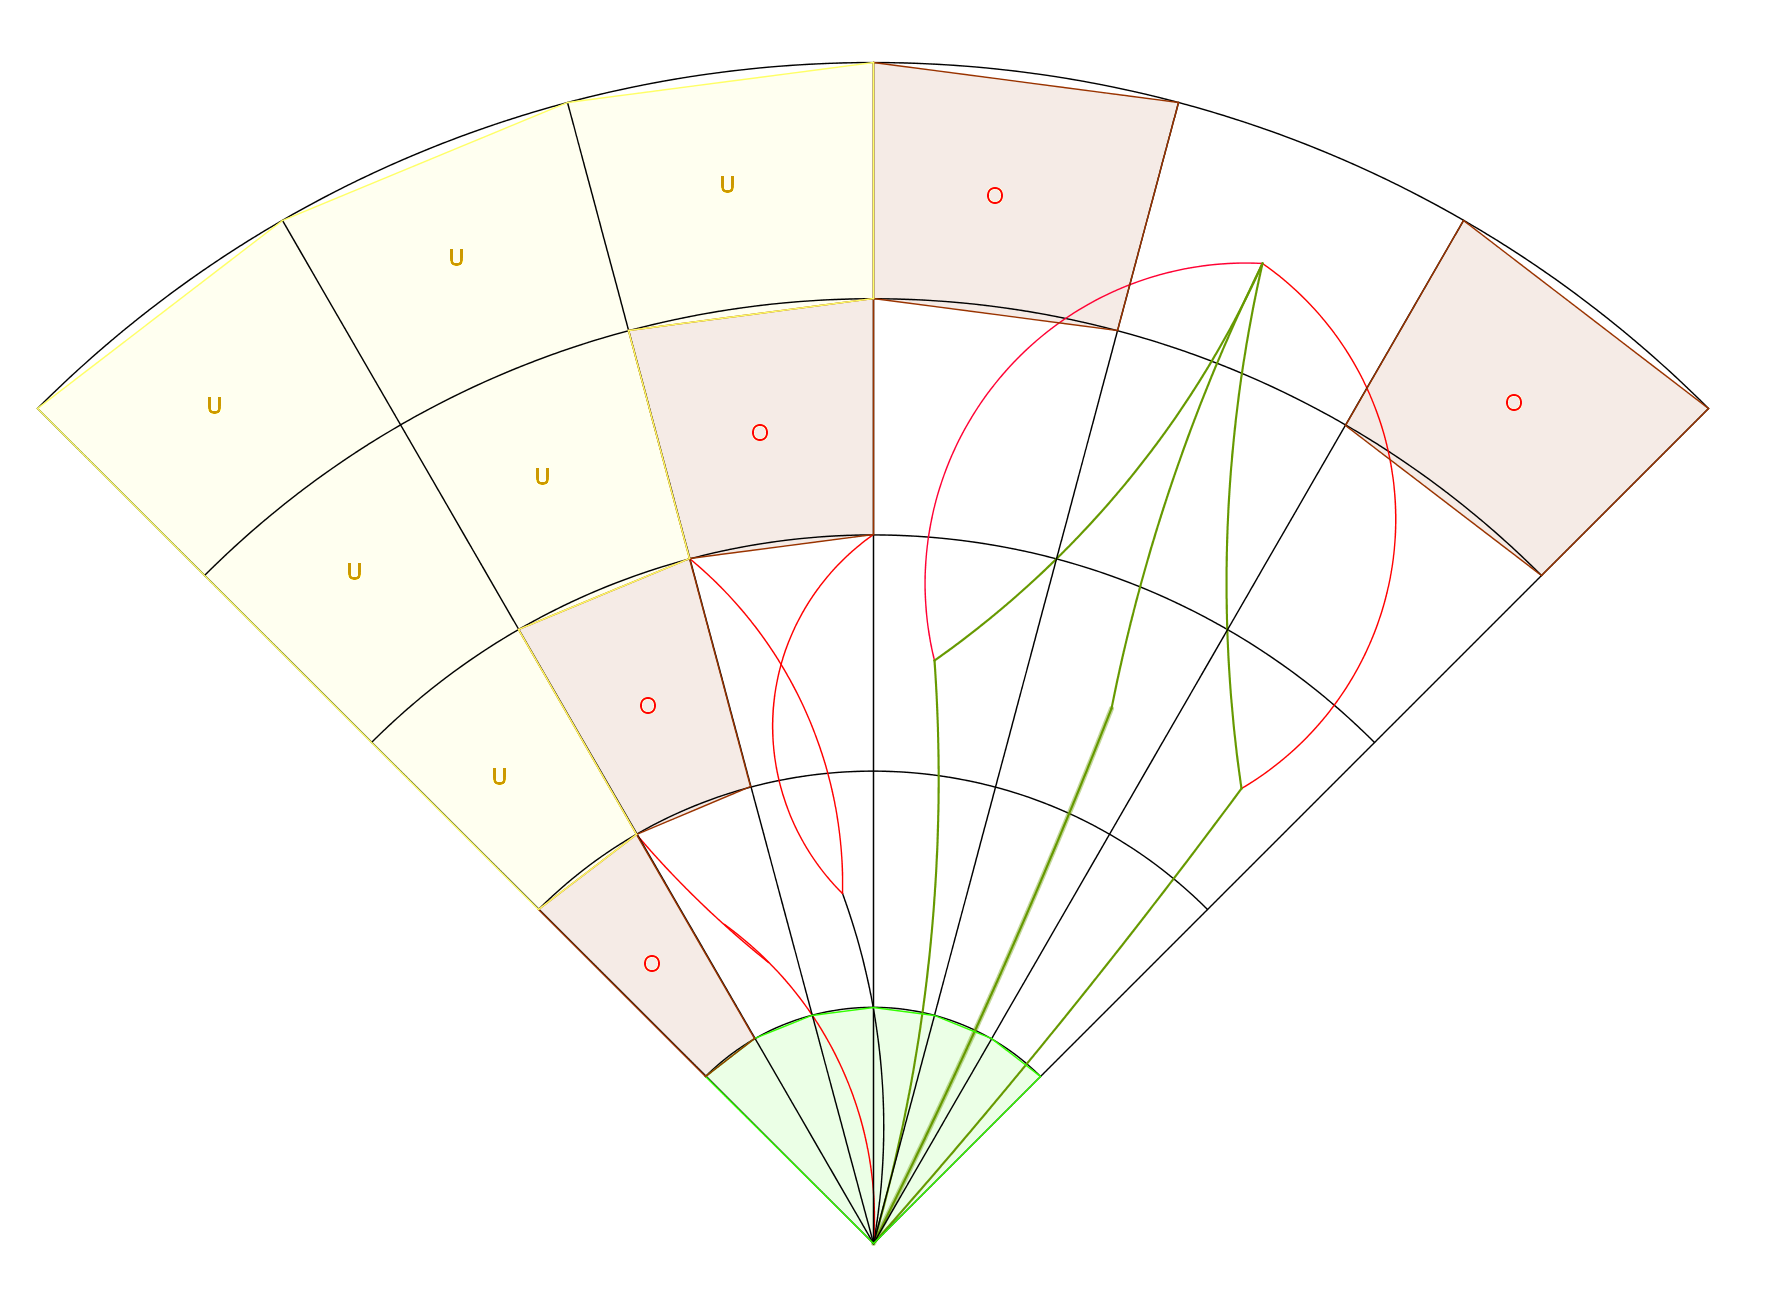
\includegraphics[width=0.9\linewidth]{\FIGDIR/CA003SurveyOfVacantSpace} 
            \caption{Trajectories safety evaluation.}
            \label{fig:trajectoriesSafetyEvaluationAvoidanceGrid}
        \end{subfigure}
        \begin{subfigure}{0.48\textwidth}
            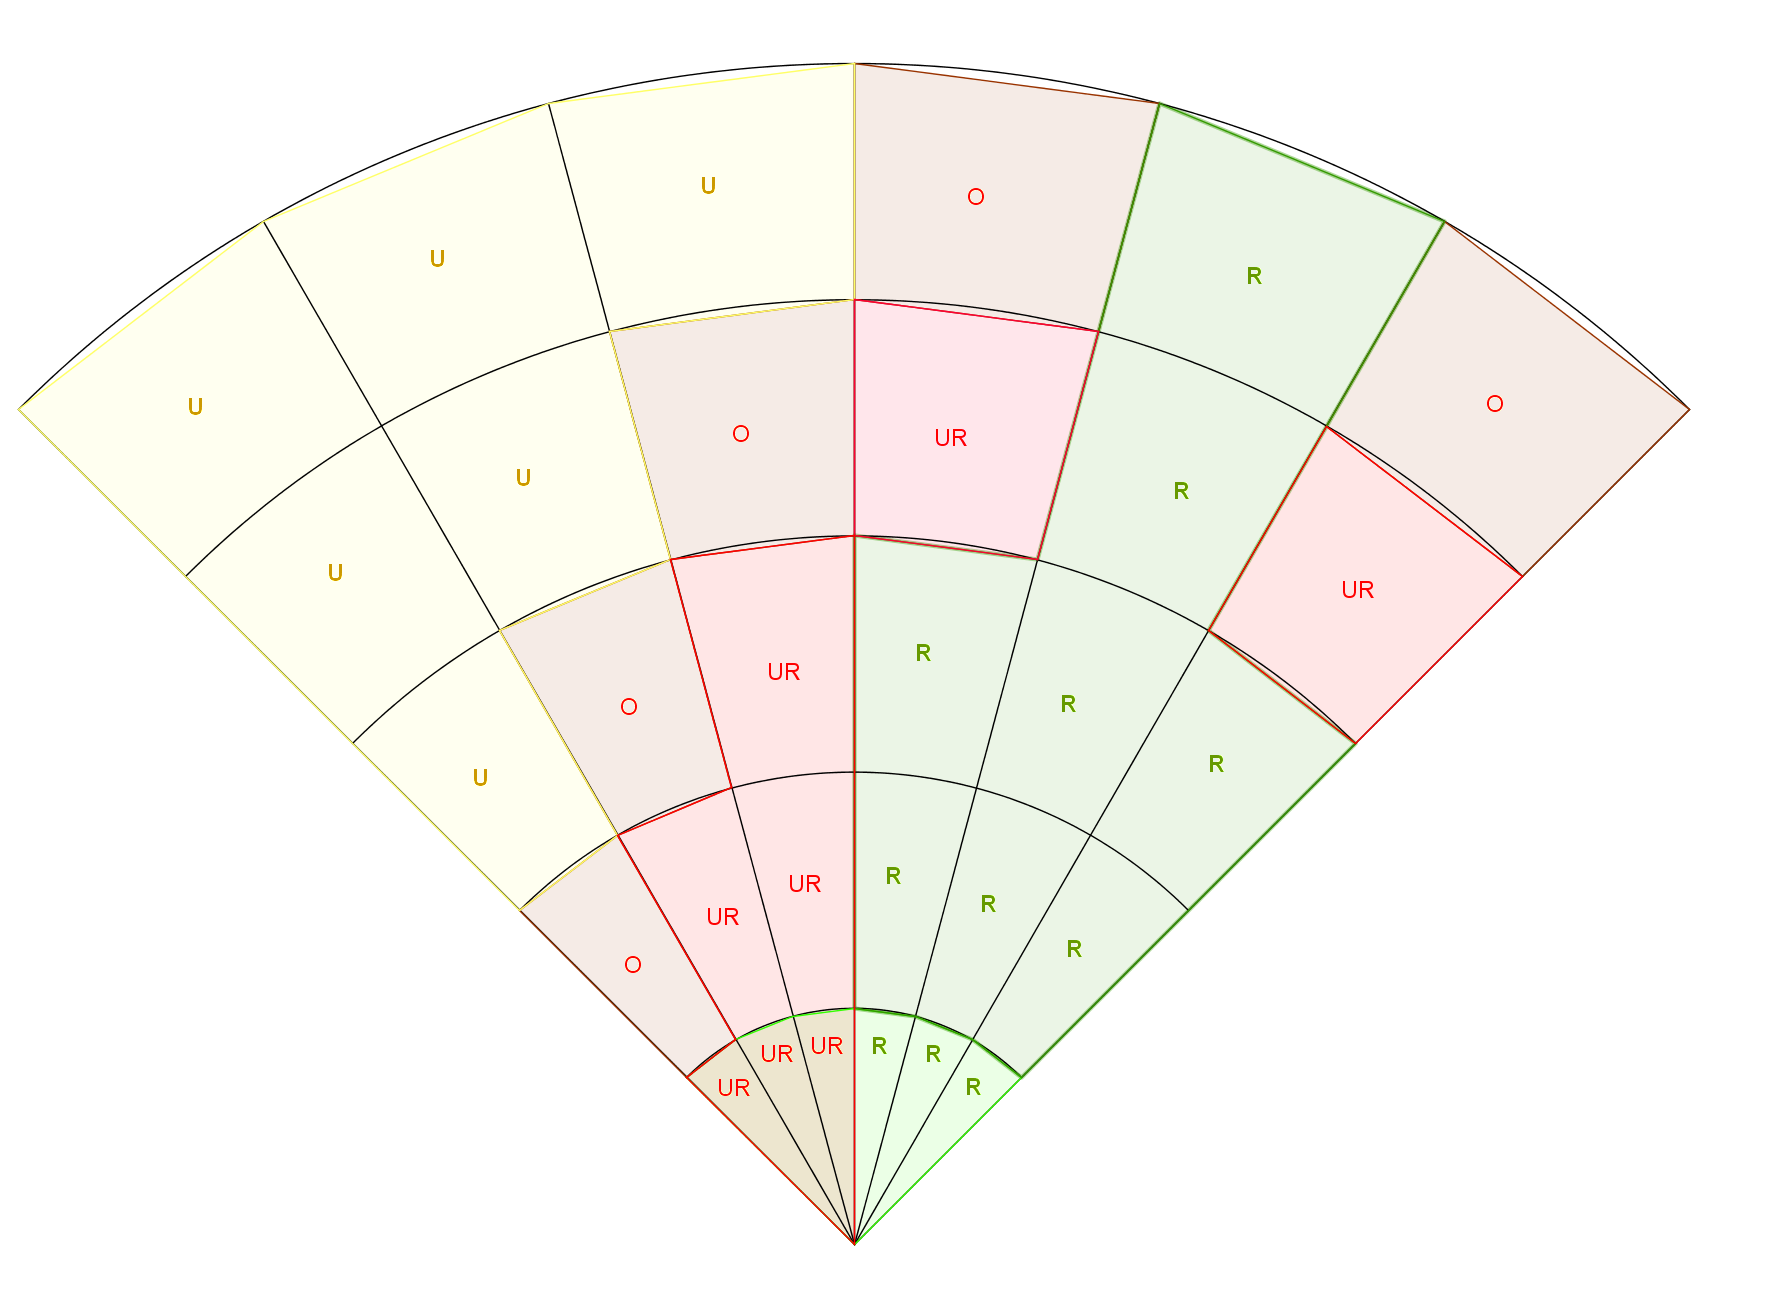
\includegraphics[width=0.9\linewidth]{\FIGDIR/CA004ReachableSpaceAssesment} 
            \caption{Reachibility evaluation.}
            \label{fig:reachibilityAssessmentAvoidanceGrid}
        \end{subfigure}
        \caption{Significant steps of \emph{Avoidance grid run} (inner loop).}
        \label{fig:significantStepsofAvoidanceGridRun}
    \end{figure}

